\documentclass{standalone}
\usepackage{tikz}
\usetikzlibrary{shapes.geometric, arrows}

\tikzstyle{startstop} = [rectangle, rounded corners, minimum width=3cm, minimum height=1cm,text centered, draw=black, fill=red!30]
\tikzstyle{process} = [rectangle, minimum width=3cm, minimum height=1cm, text centered, draw=black, fill=orange!30]
\tikzstyle{arrow} = [thick,->,>=stealth]

\begin{document}

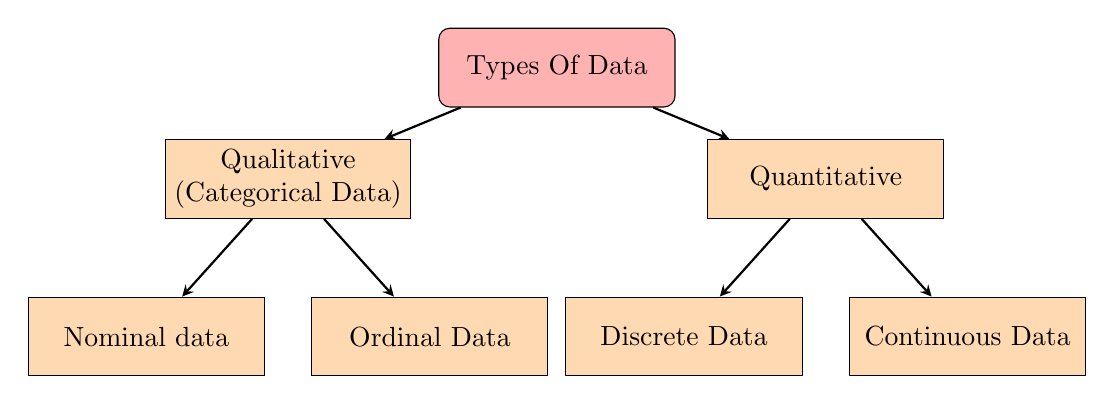
\begin{tikzpicture}[node distance=2cm]

\node (start) [startstop] {Types Of Data};
\node (cat) [process, align=center, below left of=start, xshift=-2cm] {Qualitative \\ (Categorical Data)};
\node (quant) [process, below right of=start, xshift=2cm] {Quantitative};
\node (nominal) [process, below of=cat, xshift=-1.8cm] {Nominal data};
\node (ordinal) [process, below of=cat, xshift=1.8cm] {Ordinal Data};
\node (discrete) [process, below of=quant, xshift=-1.8cm] {Discrete Data};
\node (continuous) [process, below of=quant, xshift=1.8cm] {Continuous Data};

\draw [arrow] (start) -- (cat);
\draw [arrow] (start) -- (quant);
\draw [arrow] (cat) -- (nominal);
\draw [arrow] (cat) -- (ordinal);
\draw [arrow] (quant) -- (discrete);
\draw [arrow] (quant) -- (continuous);

\end{tikzpicture}

\end{document}
